\chapter{Экспериментальная часть}

В данном разделе описаны замерные эксперименты и представлены результаты исследования.

\section{Технические характеристики}
Технические характеристики устройства, на котором выполнялся эксперимент \cite{bib:5}:
\begin{itemize}
	\item 8 ГБ оперативной памяти;
	\item процессор Apple M2;
    \item операционная система macOS Ventura 13.0.
\end{itemize}

\section{Измерение процессорного времени выполнения реализаций алгоритмов}

Для измерения процессорного времени выполнения реализаций алгоритмов была использована функция языка $C$~---~$clock\_gettime$, которая позволяет получить текущее процессорное время в наносекундах \cite{bib:6}.

В таблице \ref{table:time} представлены результаты измерений процессорного времени выполнения в зависимости от длины строки. На рисунке \ref{img:time} представлена зависимость времени выполнения от длины строк.

\begin{table}[h]
  \caption{\label{table:time} Результаты замеров процессорного времени (в нс)}
  \begin{center}
    \begin{tabular}{|r|r|r|r|r|}
      \hline
      Длина & Лев. & Дам.-Лев. & Дам.-Лев. рек. & Дам.-Лев. рек. кеш. \\ \hline
      1 & 480 & 360 & 440 & 730 \\ \hline
      2 & 650 & 710 & 1890 & 1730 \\ \hline
      3 & 1200 & 1230 & 8190 & 2960 \\ \hline
      4 & 1830 & 1650 & 87720 & 8030 \\ \hline
      5 & 3370 & 3330 & 289660 & 7500 \\ \hline
      6 & 2940 & 2870 & 929850 & 7670 \\ \hline
      7 & 2760 & 2760 & 4643940 & 9850 \\ \hline
      8 & 3630 & 3640 & 25635910 & 14060 \\ \hline
      10 & 5640 & 5630 & 784663680 & 20660 \\ \hline
    \end{tabular}
  \end{center}
\end{table}

\newpage

\noindent
\begin{figure}[h!]
	\centering
    \includegraphics[width=0.75\linewidth]{../data/time}
    \caption{Результаты замеров времени}
    \label{img:time}
\end{figure}

Так как на этом масштабе не видна разница между реализациями матричных алгоритмов Левенштейна и Дамерау-Левенштейна, то на рисунке \ref{img:time_matrix} представлена зависимость времени выполнения от длин строк для данных двух алгоритмов на более крупной выборке.

\noindent
\begin{figure}[h!]
	\centering
    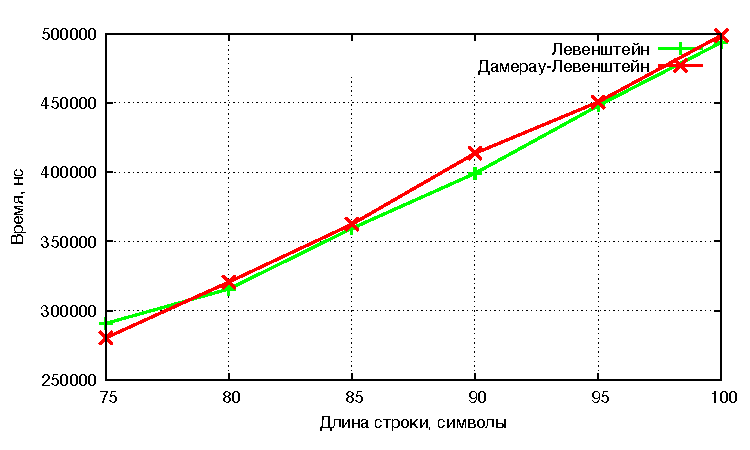
\includegraphics[width=0.75\linewidth]{../data/time_matrix}
    \caption{Результаты замеров времени для матричных реализаций}
    \label{img:time_matrix}
\end{figure}

\newpage


\section{Измерение объёма потребляемой памяти реализаций алгоритмов}

В таблице \ref{table:memory} представлены результаты измерения потребляемой памяти в зависимости от длины строки. На рисунке \ref{img:memory} представлена зависимость потребляемой памяти от длины строк.

\begin{table}[h]
  \caption{\label{table:memory} Результаты замеров потребляемой памяти (в байтах)}
  \begin{center}
    \begin{tabular}{|r|r|r|r|r|}
      \hline
      Длина & Лев (м) & Дам-Лев & Дам-Лев рек. & Дам-Лев рек. кеш. \\ \hline
      1 & 252 & 252 & 144 & 356 \\ \hline
      2 & 281 & 281 & 288 & 561 \\ \hline
      3 & 312 & 312 & 432 & 768 \\ \hline
      4 & 345 & 345 & 576 & 977 \\ \hline
      5 & 380 & 380 & 720 & 1188 \\ \hline
      6 & 417 & 417 & 864 & 1401 \\ \hline
      7 & 456 & 456 & 1008 & 1616 \\ \hline
      8 & 497 & 497 & 1152 & 1833 \\ \hline
      10 & 585 & 585 & 1440 & 2273 \\ \hline
    \end{tabular}
  \end{center}
\end{table}

\newpage


\noindent
\begin{figure}[t!]
	\centering
    \includegraphics[width=0.75\linewidth]{../data/memory.pdf}
    \caption{Результаты замеров памяти}
    \label{img:memory}
\end{figure}

\newpage